\chapter{Projektmanagement}
\section{Entscheidung}
Die Entscheidung der Projektmanagementmethode ist sehr wichtig und sollte sorgfältig gemacht werden. Sollte eine Methode falsch angewandt werden, kann sie das Team verlangsamen und bei der Arbeit hindern. Bei dieser Entscheidung hilft die Stacey Matrix.

\begin{wrapfigure}[15]{r}[0pt]{0.5\textwidth}
  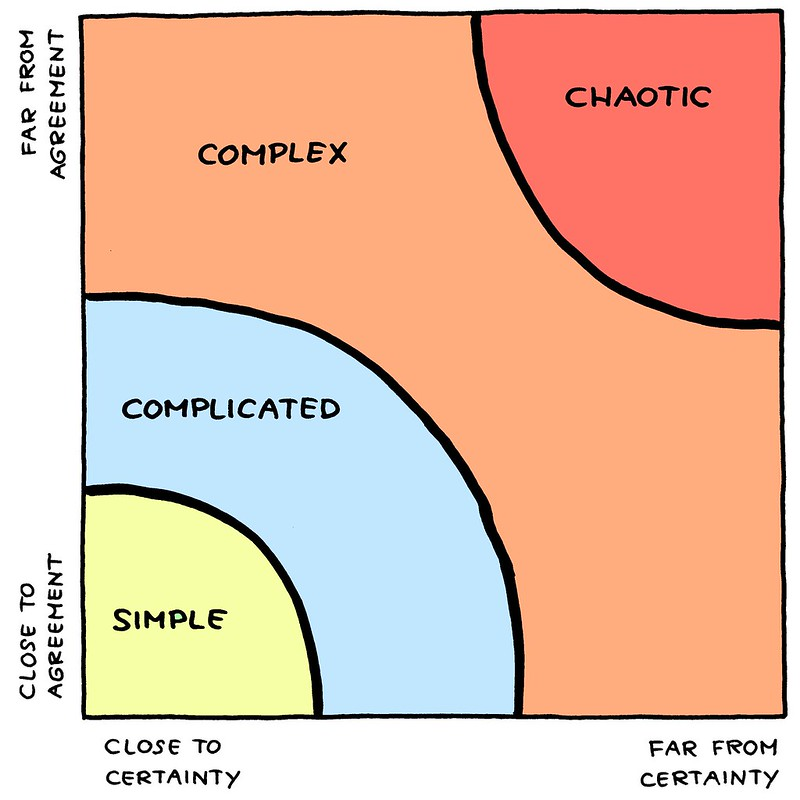
\includegraphics[width=0.9\linewidth]{./images/stacey_matrix}
  \caption[\href{https://blog.ordix.de/welches-vorgehen-eignet-sich-fuer-mein-projekt}{Stacey Matrix Grafik von Jurgen Appello.}]{Stacey Matrix}
  \label{fig:stacey}
\end{wrapfigure}\leavevmode

Die x-Achse beschreibt die Verständlichkeit des Auftrags. Das heisst, ob alle Anforderungen gegeben sind oder noch welche zu einem späteren Zeitpunkt dazu kommen können. Die y-Achse beschreibt dagegen, wie deutlich der Weg zu diesen Anforderungen ist. Dabei fragt sich zum Beispiel, wie man den Auftrag mit dieser Programmiersprache lösen kann.
\newline
Die ganze Auswertung beruht auf Schätzungen. Diese subjektiven Beobachtungen werden allerdings präziser, je mehr Berufserfahrung man sammelt.
\newline
In der Abbildung \ref*{fig:stacey} gibt es vier Abschnitte. Je Kategorie sollte man eine andere Projektmanagementmethode anwenden.
\newpage
\begin{itemize}
  \item \textbf{Simpel} - Das Ziel und der Weg sind klar. In diesem Fall sollte das Wasserfallmodell oder eine ähnliche Methode gewählt werden.
  \item \textbf{Kompliziert} - Sollte entweder das Ziel oder noch nicht ganz klar sein, sollte man Kanban anwenden.
  \item \textbf{Komplex} - Sind beide Achsen unklar oder ändern sich Kriterien, sollte etwas Agiles wie Scrum gewählt werden. Eine Methode wie diese  eignet sich für wechselnde Anforderungen.
  \item \textbf{Chaotisch} - Das Ziel und der Weg sind unklar. In diesem Fall sollte das Projekt noch nicht gestartet werden. Stattdessen sollte für mehr Klarheit bezüglich Weg und Ziel geschaffen werden. 
\end{itemize}

\section{Wasserfallmodell}

\begin{figure}[!ht]
  \centering
  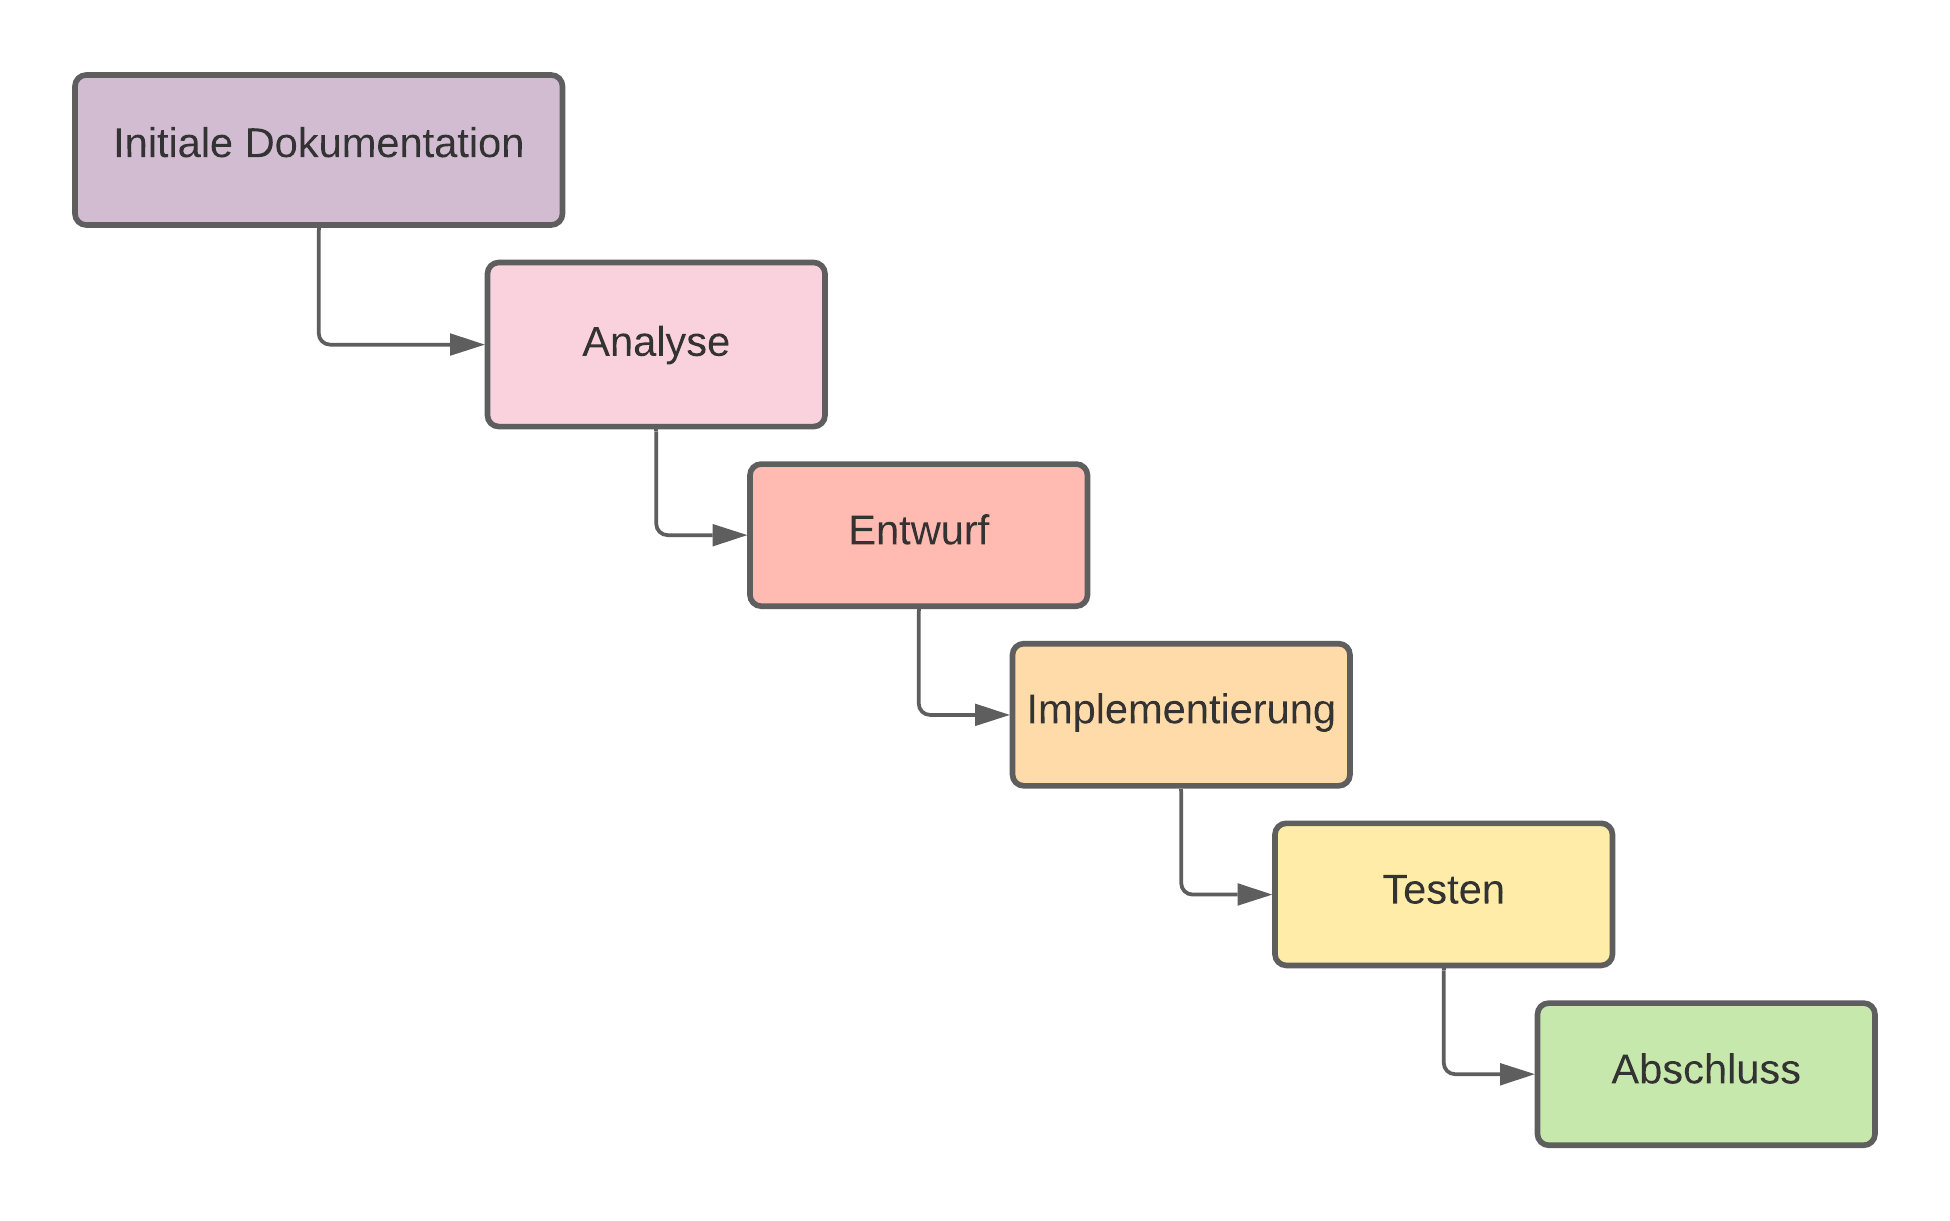
\includegraphics[width=.95\linewidth]{./images/OSEDashboard_Wasserfall.png}
  \caption[Ein von mir mit Lucidchart erstelltes Wasserfallmodell]{Wasserfall Modell}
  \label{fig:wasserfall}
\end{figure}

Das Wasserfallmodell ist eine Abfolge sequenzieller Phase, wobei man erst mit der nächsten Stufe beginnt, wenn die davorliegende abgeschlossen ist. Dies erfordert, dass das Ziel und der Weg klar sein muss. Ein streng geregelter Arbeitsablauf mit Meilensteinen kann dadurch ermöglicht werden, was vorallem für kleine Projekte sehr nützlich ist. Dies ist auch der Grund, weshalb man sich bei dieser Arbeit für das Wasserfallmodel entschieden hat.

\subsection{Initialisierung des Dokuments}

Als Erstes soll das Dokument für die kommenden Arbeitstage so vorbereitet werden, damit zukünftige zeitaufwendige Anpassungen vermeiden werden können. Zuerst soll die LaTeX-Vorlage nochmals angesehen werden, um sicherzugehen, dass alles stimmt und richtig konfiguriert ist. Danach sollten essenzielle Bestandteile wie der detaillierte Zeitplan, das Arbeitsjournal und der obligatorische Teil erstellt werden.

\subsection{Analyse}

Nachdem die Initialisierung komplett abgeschlossen ist, geht es an die Analyse. Diese beinhaltet unter Anderem eine Systembeschreibung, ein Ist/Soll-Vergleich, Konzepte wie die Arbeitsergebnisse gesichert werden und die OAuth2-Strategie. Ersteres beschreibt, wie genau unser Netilion-Ökosystem funktioniert und wie dieses Projekt integriert werden soll. Der Ist/Soll-Vergleich zeigt nochmals die zu erarbeitende Lösung auf und wie sie sich von dem bereits existierenden Produkt differenziert. Die OAuth2-Strategie soll genau beschreiben, wie der Anmeldeprozess abläuft und was ihn sicher macht.
\newline
Ausserdem enthalten sind Personas und detaillierte User-Stories. Diese werden gebildet, indem die Anforderung des Auftraggebers unterteilt werden, damit sich der Entwickler auf einzelne Entwicklungsabschnitte konzentrieren kann und der Fortschritt messbarer ist.

\subsubsection{User-Stories}

Die User Story beschreibt in kurzer Form eine Anforderung einer Anspruchsgruppe an die Software. Dabei soll geklärt werden, \textbf{wer} welche \textbf{Funktionalität} aus welchem \textbf{Grund} implementiert haben möchte\cite{atlassian_2021_user}. Ohne dabei zu sehr in technische Details zu gehen, beschreibt sie, was genau von der Software gefordert ist. Dadurch wird die Absprache mit den Anspruchsgruppen erleichter. Wie die Anforderungen implementiert werden, liegt im Ermessen des Entwicklers. Sehr oft wird diese kurze Beschreibung als Titel für eine Story im Projektmanagementtool angegeben.

\textbf{Beispiel einer User Story:}
\newline
\textbf{Aufbau:} Als \textit{<Anspruchsgruppe>} möchte ich \textit{<Feature>}, damit \textit{<Anwendungsfall>} erreicht wird.
\linebreak
\textbf{Beispiel:} Als \textit{Nutzer} möchte ich, dass \textit{die ne107 Werte grafisch dargestellt werden} , damit \textit{ich die Status der Messgeräte direkt sehen kann}.

\subsection{Entwurf}

In der Entwurfsphase wird der genaue Lösungsweg ermittelt. Der Entwickler beschreibt, wie er mit welchen technischen Mitteln die zuvor definierten Ziele erreichen kann. Dazu gehören Schnittstellen, Bibliotheken, Datenbank und Weiteres. Das Ergebnis dieser Phase ist ein ausgearbeitetes User Interface/User Experience Design, genaue Pläne, wie die Software aufgebaut werden soll und das Testkonzept.

\subsection{Implementierung}

In diesem Abschnitt gilt es, die dokumentierten Anforderungen mit den gewählten Technologien umzusetzen. Dabei sollen die User-Stories und Testfälle der vorherigen Kapiteln berüclsichtigt werden.
\newline
Nachdem eine Story abgeschlossen ist, wird die Änderung auf einen Branch gepusht und automatisch deployed. So können die Anspruchsgruppen dem Entwickler zeitnahe Rückmeldungen geben. Das Produkt der späteren Implementierungsphase ist die fertige Software.


\subsection{Testen}

In dieser Phase wird nochmals sorgfältig durchgegangen, ob alle Kriterien erfüllt wurden und ob die Tests wie gewünscht ablaufen. Stimmt das Ergebnis mit den gesetzten Erwartungen, gilt die Software als fertiggestellt.

\subsection{Abschluss}

Nachdem alle Ziele erreicht und mit dem Testprotokoll verifiziert wurden, wird die verbleibende Zeit für die Überarbeitung der Dokumentation eingesetzt werden. Anschliesend soll die IPA am 14.04.2021 abgegeben werden.